% Options for packages loaded elsewhere
\PassOptionsToPackage{unicode}{hyperref}
\PassOptionsToPackage{hyphens}{url}
%
\documentclass[
]{article}
\usepackage{amsmath,amssymb}
\usepackage{iftex}
\ifPDFTeX
  \usepackage[T1]{fontenc}
  \usepackage[utf8]{inputenc}
  \usepackage{textcomp} % provide euro and other symbols
\else % if luatex or xetex
  \usepackage{unicode-math} % this also loads fontspec
  \defaultfontfeatures{Scale=MatchLowercase}
  \defaultfontfeatures[\rmfamily]{Ligatures=TeX,Scale=1}
\fi
\usepackage{lmodern}
\ifPDFTeX\else
  % xetex/luatex font selection
\fi
% Use upquote if available, for straight quotes in verbatim environments
\IfFileExists{upquote.sty}{\usepackage{upquote}}{}
\IfFileExists{microtype.sty}{% use microtype if available
  \usepackage[]{microtype}
  \UseMicrotypeSet[protrusion]{basicmath} % disable protrusion for tt fonts
}{}
\makeatletter
\@ifundefined{KOMAClassName}{% if non-KOMA class
  \IfFileExists{parskip.sty}{%
    \usepackage{parskip}
  }{% else
    \setlength{\parindent}{0pt}
    \setlength{\parskip}{6pt plus 2pt minus 1pt}}
}{% if KOMA class
  \KOMAoptions{parskip=half}}
\makeatother
\usepackage{xcolor}
\usepackage[margin=1in]{geometry}
\usepackage{longtable,booktabs,array}
\usepackage{calc} % for calculating minipage widths
% Correct order of tables after \paragraph or \subparagraph
\usepackage{etoolbox}
\makeatletter
\patchcmd\longtable{\par}{\if@noskipsec\mbox{}\fi\par}{}{}
\makeatother
% Allow footnotes in longtable head/foot
\IfFileExists{footnotehyper.sty}{\usepackage{footnotehyper}}{\usepackage{footnote}}
\makesavenoteenv{longtable}
\usepackage{graphicx}
\makeatletter
\def\maxwidth{\ifdim\Gin@nat@width>\linewidth\linewidth\else\Gin@nat@width\fi}
\def\maxheight{\ifdim\Gin@nat@height>\textheight\textheight\else\Gin@nat@height\fi}
\makeatother
% Scale images if necessary, so that they will not overflow the page
% margins by default, and it is still possible to overwrite the defaults
% using explicit options in \includegraphics[width, height, ...]{}
\setkeys{Gin}{width=\maxwidth,height=\maxheight,keepaspectratio}
% Set default figure placement to htbp
\makeatletter
\def\fps@figure{htbp}
\makeatother
\setlength{\emergencystretch}{3em} % prevent overfull lines
\providecommand{\tightlist}{%
  \setlength{\itemsep}{0pt}\setlength{\parskip}{0pt}}
\setcounter{secnumdepth}{-\maxdimen} % remove section numbering
\usepackage{longtable}
\usepackage{booktabs}
\usepackage{float}
\usepackage{caption}
\usepackage{changepage}
\usepackage{booktabs}
\usepackage{longtable}
\usepackage{array}
\usepackage{multirow}
\usepackage{wrapfig}
\usepackage{float}
\usepackage{colortbl}
\usepackage{pdflscape}
\usepackage{tabu}
\usepackage{threeparttable}
\usepackage{threeparttablex}
\usepackage[normalem]{ulem}
\usepackage{makecell}
\usepackage{xcolor}
\ifLuaTeX
  \usepackage{selnolig}  % disable illegal ligatures
\fi
\usepackage{bookmark}
\IfFileExists{xurl.sty}{\usepackage{xurl}}{} % add URL line breaks if available
\urlstyle{same}
\hypersetup{
  pdftitle={Simulation Analysis},
  pdfauthor={Sophie Litschwartz},
  hidelinks,
  pdfcreator={LaTeX via pandoc}}

\title{Simulation Analysis}
\author{Sophie Litschwartz}
\date{2024-08-09}

\begin{document}
\maketitle

\subsection{Introduction and Overview}\label{introduction-and-overview}

*I need to write this once I figure out what goes here

\subsection{Data Generating Process}\label{data-generating-process}

The simulations are a fully factored experiment.

\textbf{Block Level Fixed Covariates}\\
Number of Blocks: 5; ATE: .2; ICC: .2; Average Number of Observations
Per Cluster: 20; Proportion of Clusters Treated: .5 (this is fixed
across blocks); Number of District Level Covariates: 0

\textbf{Block Level Varying Covariates (Factors that are varied across
simulations)}

Three groups of block level parameters Blocks all the same, Blocks all
messy, and Blocks all reasonable

Blocks all the same: How much do number clusters per block vary (size
ratio)?: 0 (none); How much does the size of the cluster vary (size
ratio)? 0 (none); ATE SD: 0; Correlation Between Treatment Effect and
Cluster Size: 0; Correlation Between Average Number of Observations Per
Cluster and Total Number of Clusters: 0; Correlation of Proportion of
Clusters Treated per Block and Impact: 0; Correlation Between Outcome
Intercept and Cluster Size: 0

Blocks all messy: How much do number clusters per block vary (size
ratio)?: 1.3 (big) ; How much does the size of the cluster vary (size
ratio)? 1.3 (big); ATE SD: .6; Correlation Between Treatment Effect and
Cluster Size: .8; Correlation Between Average Number of Observations Per
Cluster and Total Number of Clusters: .8; Correlation of Proportion of
Clusters Treated per Block and Impact: .8; Correlation Between Outcome
Intercept and Cluster Size: .8

Blocks all reasonable: How much do number clusters per block vary (size
ratio)?: .4 (average); How much does the size of the cluster vary (size
ratio)? .4 (average); ATE SD: .1; Correlation Between Treatment Effect
and Cluster Size: .2; Correlation Between Average Number of Observations
Per Cluster and Total Number of Clusters: .1; Correlation of Proportion
of Clusters Treated per Block and Impact: 0; Correlation Between Outcome
Intercept and Cluster Size: .1

Each of the rest of these factors don't vary as a group but vary each
individually and are fully factored with all other factors:

Average Number of Clusters per Block: 4,8,16

\textbf{Cluster Level Varying Parameters}

Correlation of Impact and Size of Cluster: 0, .8

Cluster Level Treatment Effect Standard Deviation: 0, .3

Cluster Level ICC: 0, .2

Number of Observations Per Cluster Varies: True, False

Ratio of Size Cluster Sizes: 0, .4, 1.3

Number of School-Level Covariates: 0, 1, 5

{[}School Level Covariate R Squared is always .5{]}

\subsection{What does the bias look like for each
estimator}\label{what-does-the-bias-look-like-for-each-estimator}

The estimators that theory says should be biased are in fact much more
biased across the simulations. These boxplots are across the different
data generating processes, each dot is the mean bias across simulation
replications. The methods in light blue are the ones theory says should
be biased. I only show the finite population numbers because they are
the same as the super population results.

There are tables showing how the different simulation facets predict
bias. The regression model is how each facet of the data generating
process predicts mean bias against a methods targeted estimand. The
facets are binary indicators and are fully interacted with each other. I
ran three models: just the cluster targeted methods, just the person
targeted methods, and all methods. I don't know what to make of the
results.

To-Do: Re-write the summary section

\begin{center}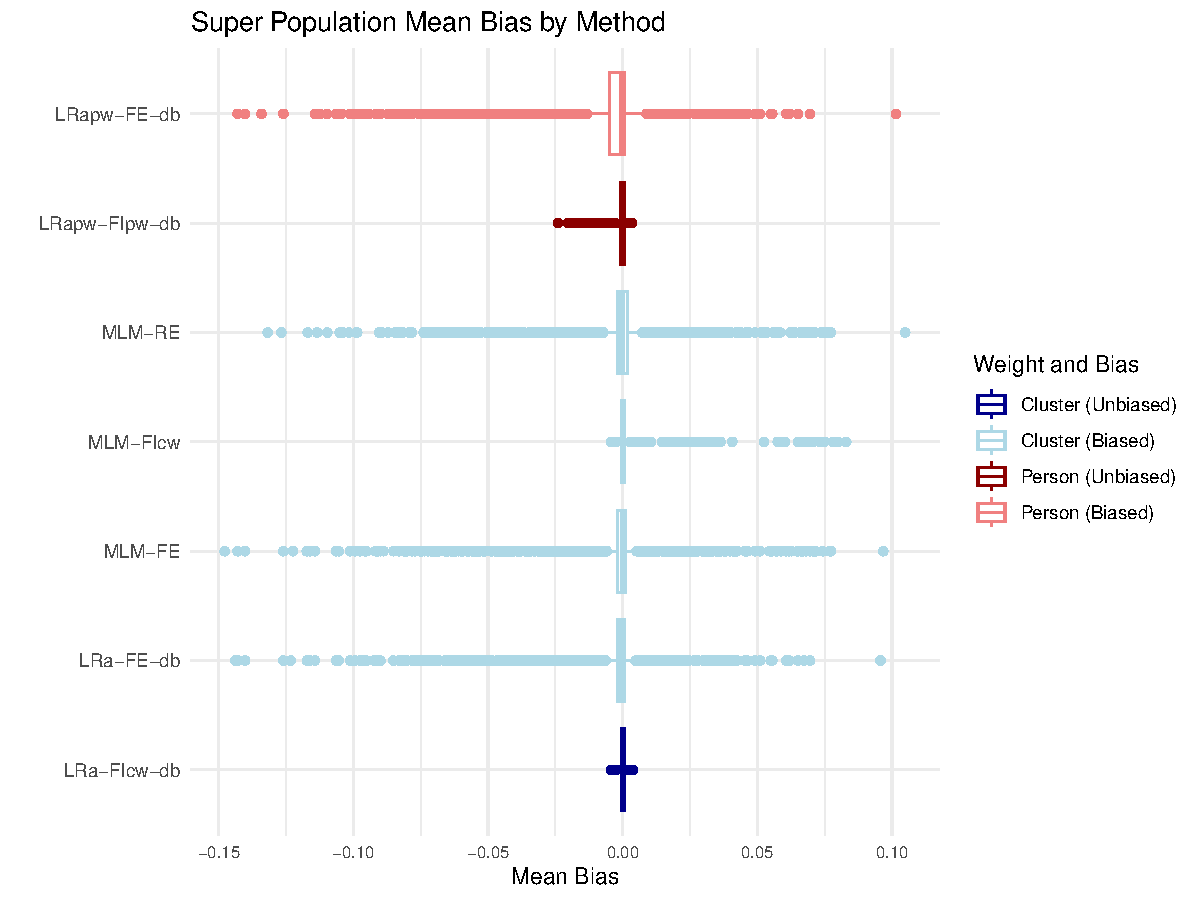
\includegraphics{Simulation-Memo-3_files/figure-latex/bias-1} \end{center}

\pagebreak

\subsubsection{The Effect of Different Data Generating Parameters on the
Magnitude of Mean
Bias}\label{the-effect-of-different-data-generating-parameters-on-the-magnitude-of-mean-bias}

\begingroup
\footnotesize

\begin{longtable}[]{@{}
  >{\raggedright\arraybackslash}p{(\columnwidth - 14\tabcolsep) * \real{0.2583}}
  >{\centering\arraybackslash}p{(\columnwidth - 14\tabcolsep) * \real{0.1000}}
  >{\centering\arraybackslash}p{(\columnwidth - 14\tabcolsep) * \real{0.1167}}
  >{\centering\arraybackslash}p{(\columnwidth - 14\tabcolsep) * \real{0.1167}}
  >{\centering\arraybackslash}p{(\columnwidth - 14\tabcolsep) * \real{0.1333}}
  >{\centering\arraybackslash}p{(\columnwidth - 14\tabcolsep) * \real{0.0917}}
  >{\centering\arraybackslash}p{(\columnwidth - 14\tabcolsep) * \real{0.0917}}
  >{\centering\arraybackslash}p{(\columnwidth - 14\tabcolsep) * \real{0.0917}}@{}}
\toprule\noalign{}
\begin{minipage}[b]{\linewidth}\raggedright
Term
\end{minipage} & \begin{minipage}[b]{\linewidth}\centering
LRa-FE-db
\end{minipage} & \begin{minipage}[b]{\linewidth}\centering
LRa-FIcw-db
\end{minipage} & \begin{minipage}[b]{\linewidth}\centering
LRapw-FE-db
\end{minipage} & \begin{minipage}[b]{\linewidth}\centering
LRapw-FIpw-db
\end{minipage} & \begin{minipage}[b]{\linewidth}\centering
MLM-FE
\end{minipage} & \begin{minipage}[b]{\linewidth}\centering
MLM-FIcw
\end{minipage} & \begin{minipage}[b]{\linewidth}\centering
MLM-RE
\end{minipage} \\
\midrule\noalign{}
\endhead
\bottomrule\noalign{}
\endlastfoot
(Intercept) & .007. & \textless.001* & .009* & .002*** & .009* & .005**
& .009* \\
block\_typeS & \textless.001 & \textless.001 & \textless.001 &
\textless.001 & \textless.001 & \textless.001 & .001 \\
block\_typeL & .036*** & \textless.001 & .037*** & \textless.001 &
.042*** & .001 & .036*** \\
J.barS & -.003 & \textless.001 & -.003 & \textless.001 & -.004 & -.001 &
-.005 \\
J.barL & -.002 & \textless.001 & -.002 & .001** & -.004 & -.002 &
-.003 \\
size.impact.cor.schoolL & -.005 & \textless.001 & -.006* & -.003*** &
-.009** & -.008*** & -.008** \\
sd.schoolL & \textless.001 & \textless.001 & -.002 & -.002*** & -.005 &
-.008*** & -.007* \\
ICC.schoolL & -.007* & .001*** & -.008* & .001** & \textless.001 &
.010*** & \textless.001 \\
variable.nTRUE & -.006. & \textless.001 & -.007* & -.002*** & -.010** &
-.008*** & -.009** \\
cv.schoolS & -.006 & \textless.001 & -.006. & -.001*** & -.008. & -.004*
& -.008* \\
cv.schoolL & -.001 & \textless.001 & -.002 & -.002*** & -.005 & -.009***
& -.007. \\
num.cov.schoolS & -.005 & \textless.001 & -.005 & \textless.001 & -.005
& \textless.001 & -.004 \\
num.cov.schoolL & .001 & \textless.001 & .001 & \textless.001 &
\textless.001 & \textless.001 & .001 \\
block\_typeS:J.barS & \textless.001 & \textless.001 & \textless.001 &
\textless.001 & \textless.001 & \textless.001 & -.002 \\
block\_typeL:J.barS & \textless.001 & \textless.001 & \textless.001 &
\textless.001 & -.001 & \textless.001 & .001 \\
block\_typeS:J.barL & \textless.001 & \textless.001 & \textless.001 &
\textless.001 & \textless.001 & \textless.001 & -.003 \\
block\_typeL:J.barL & -.001 & \textless.001 & \textless.001 &
\textless.001 & -.001 & \textless.001 & .004 \\
block\_typeS: size.impact.cor.schoolL & \textless.001 & \textless.001. &
\textless.001 & \textless.001 & \textless.001 & \textless.001 &
\textless.001 \\
block\_typeL: size.impact.cor.schoolL & -.006** & \textless.001 &
-.007** & \textless.001 & -.011*** & \textless.001 & -.009*** \\
block\_typeS:sd.schoolL & \textless.001 & \textless.001 & \textless.001
& \textless.001 & \textless.001 & \textless.001 & \textless.001 \\
block\_typeL:sd.schoolL & -.002 & \textless.001 & -.002 & \textless.001
& -.007** & \textless.001 & -.007** \\
block\_typeS:ICC.schoolL & \textless.001 & \textless.001 & \textless.001
& \textless.001 & \textless.001 & \textless.001 & .002 \\
block\_typeL:ICC.schoolL & -.005* & \textless.001 & -.004* &
\textless.001 & -.003 & \textless.001 & -.005* \\
block\_typeS: variable.nTRUE & \textless.001 & \textless.001 &
\textless.001 & \textless.001 & \textless.001 & \textless.001 &
\textless.001 \\
block\_typeL: variable.nTRUE & .003 & \textless.001 & .001 &
\textless.001 & -.002 & \textless.001 & -.002 \\
block\_typeS:cv.schoolS & \textless.001 & \textless.001 & \textless.001
& \textless.001 & \textless.001 & \textless.001 & \textless.001 \\
block\_typeL:cv.schoolS & .003 & \textless.001 & .002 & \textless.001 &
.001 & \textless.001 & \textless.001 \\
block\_typeS:cv.schoolL & \textless.001 & \textless.001 & \textless.001
& \textless.001 & \textless.001 & \textless.001 & \textless.001 \\
block\_typeL:cv.schoolL & .003 & \textless.001 & .001 & \textless.001 &
-.003 & \textless.001 & -.004 \\
block\_typeS: num.cov.schoolS & \textless.001 & \textless.001 &
\textless.001 & \textless.001 & \textless.001 & \textless.001 &
\textless.001 \\
block\_typeL: num.cov.schoolS & -.003 & \textless.001 & -.003 &
\textless.001 & -.003 & \textless.001 & -.002 \\
block\_typeS: num.cov.schoolL & \textless.001 & \textless.001 &
\textless.001 & \textless.001 & \textless.001 & \textless.001 & .001 \\
block\_typeL: num.cov.schoolL & -.001 & \textless.001 & -.002 &
\textless.001 & -.001 & \textless.001 & .001 \\
J.barS: size.impact.cor.schoolL & .002 & \textless.001 & .002 &
\textless.001 & .003 & .001 & .002 \\
J.barL: size.impact.cor.schoolL & .003 & \textless.001 & .002 & -.001***
& .005. & .002 & .004 \\
J.barS:sd.schoolL & \textless.001 & \textless.001 & -.001 &
\textless.001 & .001 & .001 & .002 \\
J.barL:sd.schoolL & .001 & \textless.001 & \textless.001 & -.001*** &
.003 & .001 & .003 \\
J.barS:ICC.schoolL & .003 & \textless.001 & .003 & \textless.001 & .003
& \textless.001 & .002 \\
J.barL:ICC.schoolL & .002 & \textless.001* & .002 & \textless.001 &
\textless.001 & -.001 & \textless.001 \\
J.barS:variable.nTRUE & .003 & \textless.001 & .002 & \textless.001 &
.004 & .001 & .003 \\
J.barL:variable.nTRUE & .003 & \textless.001 & .002 & -.001*** & .005. &
.001 & .004. \\
J.barS:cv.schoolS & .002 & \textless.001 & .002 & \textless.001 & .002 &
.001 & .003 \\
J.barL:cv.schoolS & -.001 & \textless.001 & -.001 & \textless.001 &
\textless.001 & .001 & .001 \\
J.barS:cv.schoolL & -.002 & \textless.001 & -.002 & \textless.001 &
-.001 & .001 & .001 \\
J.barL:cv.schoolL & -.003 & \textless.001. & -.004 & -.001*** & -.001 &
.001 & \textless.001 \\
J.barS:num.cov.schoolS & \textless.001 & \textless.001 & \textless.001 &
\textless.001 & \textless.001 & \textless.001 & \textless.001 \\
J.barL:num.cov.schoolS & \textless.001 & \textless.001 & \textless.001 &
\textless.001 & \textless.001 & \textless.001 & -.001 \\
J.barS:num.cov.schoolL & -.003 & \textless.001 & -.003 & \textless.001 &
-.003 & \textless.001 & -.002 \\
J.barL:num.cov.schoolL & -.003 & \textless.001 & -.002 & \textless.001 &
-.004 & \textless.001 & -.005. \\
size.impact.cor.schoolL: sd.schoolL & .003 & \textless.001 & .005** &
.003*** & .010*** & .011*** & .010*** \\
size.impact.cor.schoolL: ICC.schoolL & .002 & \textless.001 & .002 &
\textless.001 & -.002 & -.006*** & -.002 \\
size.impact.cor.schoolL: variable.nTRUE & \textless.001 & \textless.001*
& .002 & .003*** & .007*** & .011*** & .007*** \\
size.impact.cor.schoolL: cv.schoolS & .002 & \textless.001 & .003 &
.001*** & .005* & .005*** & .005* \\
size.impact.cor.schoolL: cv.schoolL & .001 & \textless.001 & .003 &
.002*** & .008** & .011*** & .007** \\
size.impact.cor.schoolL: num.cov.schoolS & .001 & \textless.001 & .001 &
\textless.001 & .001 & \textless.001 & .001 \\
size.impact.cor.schoolL: num.cov.schoolL & -.001 & \textless.001 & -.001
& \textless.001 & \textless.001 & \textless.001 & -.001 \\
sd.schoolL:ICC.schoolL & \textless.001 & \textless.001 & \textless.001 &
\textless.001 & -.005* & -.006*** & -.005** \\
sd.schoolL:variable.nTRUE & .001 & \textless.001 & .003 & .003*** &
.008*** & .011*** & .008*** \\
sd.schoolL:cv.schoolS & -.003 & \textless.001 & -.002 & .001*** &
\textless.001 & .005*** & .002 \\
sd.schoolL:cv.schoolL & -.002 & \textless.001 & \textless.001 & .002***
& .006* & .011*** & .008*** \\
sd.schoolL: num.cov.schoolS & .001 & \textless.001 & .001 &
\textless.001 & .001 & \textless.001 & .002 \\
sd.schoolL: num.cov.schoolL & -.002 & \textless.001 & -.002 &
\textless.001 & -.001 & \textless.001 & \textless.001 \\
ICC.schoolL: variable.nTRUE & .004* & \textless.001 & .004* &
\textless.001 & -.001 & -.006*** & -.001 \\
ICC.schoolL:cv.schoolS & .005* & \textless.001 & .005* & \textless.001 &
.003 & -.003** & .002 \\
ICC.schoolL:cv.schoolL & .002 & \textless.001 & .002 & \textless.001 &
-.003 & -.006*** & -.003 \\
ICC.schoolL: num.cov.schoolS & .002 & \textless.001 & .003 &
\textless.001 & .002 & \textless.001 & .002 \\
ICC.schoolL: num.cov.schoolL & .001 & \textless.001 & .001 &
\textless.001 & \textless.001 & \textless.001 & .001 \\
variable.nTRUE:cv.schoolS & .001 & \textless.001 & .002 & .001*** &
.004. & .004*** & .005* \\
variable.nTRUE:cv.schoolL & .002 & \textless.001. & .003 & .003*** &
.009*** & .011*** & .010*** \\
variable.nTRUE: num.cov.schoolS & \textless.001 & \textless.001 & .001 &
\textless.001 & .001 & \textless.001 & \textless.001 \\
variable.nTRUE: num.cov.schoolL & .002 & \textless.001 & .001 &
\textless.001 & .002 & \textless.001 & \textless.001 \\
cv.schoolS: num.cov.schoolS & .005. & \textless.001 & .005. &
\textless.001 & .005. & \textless.001 & .005. \\
cv.schoolL: num.cov.schoolS & .002 & \textless.001 & .002 &
\textless.001 & .002 & \textless.001 & .002 \\
cv.schoolS: num.cov.schoolL & .002 & \textless.001 & .002 &
\textless.001 & .002 & \textless.001 & .001 \\
cv.schoolL: num.cov.schoolL & .002 & \textless.001 & .001 &
\textless.001 & .003 & \textless.001 & .002 \\
\end{longtable}

\emph{Significance: `***' 0.001 `**' 0.01 `*' 0.05 `.' 0.1} \endgroup

\begin{longtable}[]{@{}
  >{\raggedright\arraybackslash}p{(\columnwidth - 16\tabcolsep) * \real{0.1061}}
  >{\centering\arraybackslash}p{(\columnwidth - 16\tabcolsep) * \real{0.1364}}
  >{\centering\arraybackslash}p{(\columnwidth - 16\tabcolsep) * \real{0.0606}}
  >{\centering\arraybackslash}p{(\columnwidth - 16\tabcolsep) * \real{0.0909}}
  >{\centering\arraybackslash}p{(\columnwidth - 16\tabcolsep) * \real{0.0985}}
  >{\centering\arraybackslash}p{(\columnwidth - 16\tabcolsep) * \real{0.0909}}
  >{\centering\arraybackslash}p{(\columnwidth - 16\tabcolsep) * \real{0.1288}}
  >{\centering\arraybackslash}p{(\columnwidth - 16\tabcolsep) * \real{0.1894}}
  >{\centering\arraybackslash}p{(\columnwidth - 16\tabcolsep) * \real{0.0985}}@{}}
\toprule\noalign{}
\begin{minipage}[b]{\linewidth}\raggedright
met hod
\end{minipage} & \begin{minipage}[b]{\linewidth}\centering
bias.s estimand
\end{minipage} & \begin{minipage}[b]{\linewidth}\centering
J.bar
\end{minipage} & \begin{minipage}[b]{\linewidth}\centering
sd school
\end{minipage} & \begin{minipage}[b]{\linewidth}\centering
ICC school
\end{minipage} & \begin{minipage}[b]{\linewidth}\centering
cv school
\end{minipage} & \begin{minipage}[b]{\linewidth}\centering
num.cov school
\end{minipage} & \begin{minipage}[b]{\linewidth}\centering
size.impact cor.school
\end{minipage} & \begin{minipage}[b]{\linewidth}\centering
block type
\end{minipage} \\
\midrule\noalign{}
\endhead
\bottomrule\noalign{}
\endlastfoot
LRa-FE-db & -0.144 & 0 & 0 & 0 & L & L & 0 & L \\
LRa-FE-db & -0.143 & S & 0 & L & S & S & 0 & L \\
LRa-FE-db & -0.14 & 0 & L & 0 & S & L & L & L \\
LRa-FE-db & -0.126 & 0 & 0 & 0 & L & L & 0 & L \\
LRa-FE-db & -0.123 & 0 & L & L & L & L & 0 & L \\
LRapw-FE-db & -0.143 & S & 0 & L & S & S & 0 & L \\
LRapw-FE-db & -0.14 & 0 & L & 0 & S & L & L & L \\
LRapw-FE-db & -0.134 & 0 & 0 & 0 & L & L & 0 & L \\
LRapw-FE-db & -0.126 & 0 & 0 & 0 & L & L & 0 & L \\
LRapw-FE-db & -0.114 & 0 & L & 0 & 0 & 0 & 0 & L \\
MLM-FE & -0.148 & 0 & 0 & 0 & L & L & 0 & L \\
MLM-FE & -0.143 & S & 0 & L & S & S & 0 & L \\
MLM-FE & -0.14 & 0 & L & 0 & S & L & L & L \\
MLM-FE & -0.126 & 0 & 0 & 0 & L & L & 0 & L \\
MLM-FE & -0.122 & 0 & L & L & L & L & 0 & L \\
MLM-RE & -0.132 & 0 & 0 & 0 & L & L & 0 & L \\
MLM-RE & -0.127 & S & 0 & L & S & S & 0 & L \\
MLM-RE & -0.117 & 0 & L & 0 & S & L & L & L \\
MLM-RE & -0.113 & 0 & 0 & 0 & L & L & 0 & L \\
MLM-RE & -0.11 & S & L & 0 & L & 0 & 0 & L \\
\end{longtable}

\subsection{What does the RMSE look like for each
estimator}\label{what-does-the-rmse-look-like-for-each-estimator}

As far as I can tell the RMSE actually looks pretty similar across
estimators, which is consistent with the idea of there being a bias
variance trade off. Unlike with the bias, the finite population RMSEs
are fairly different from the super population RMSEs.

Like above, the boxplots are across the different data generating
processes, each dot is a mean across simulation replications. The
methods in light blue are those classified to be biased by theory. The
ratio of finite RMSE to super RMSE plots show the ratio of RMSE from the
finite population models over the super population models, and are
designed to show that these are different.

To-Do: Fix the graph to only include the core methods Re-Run the models
here

\begin{center}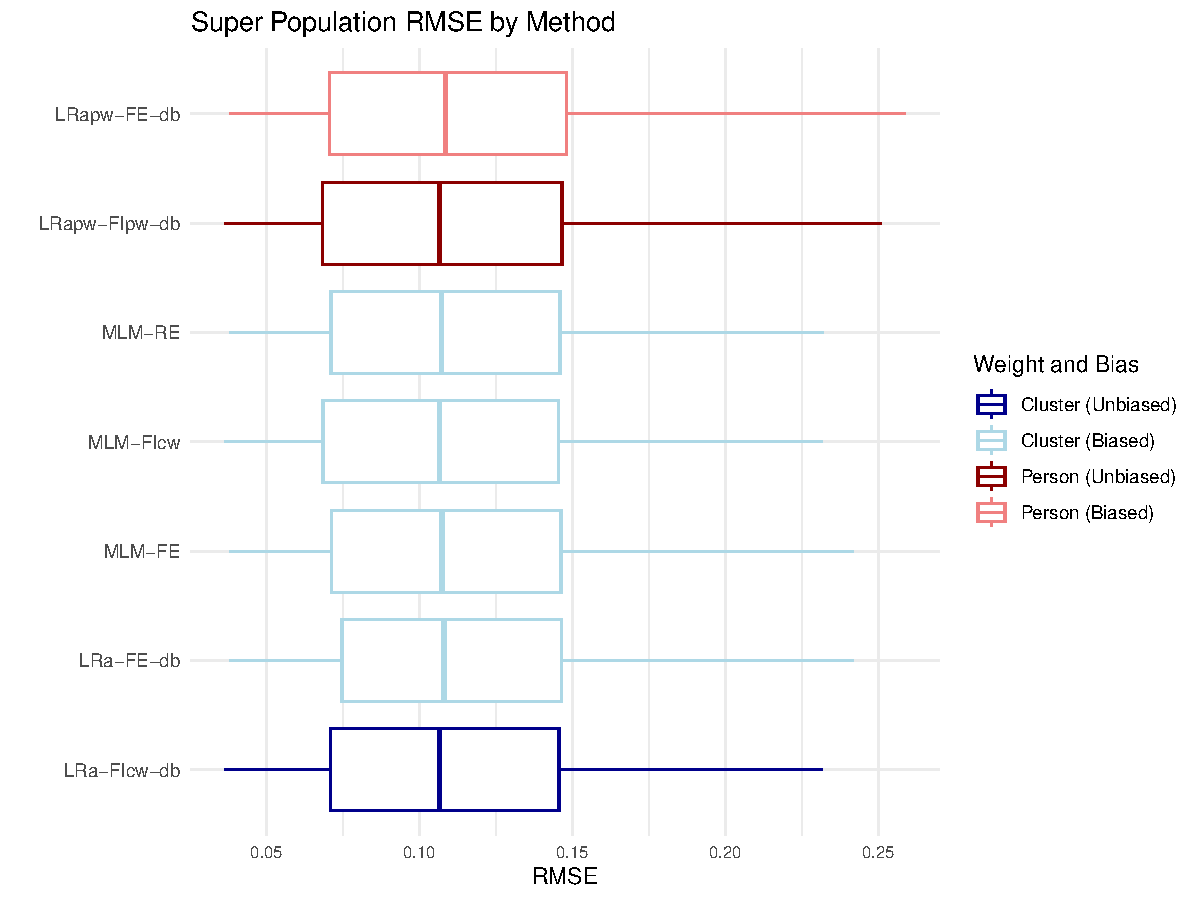
\includegraphics{Simulation-Memo-3_files/figure-latex/rmse-1} \end{center}

\begin{center}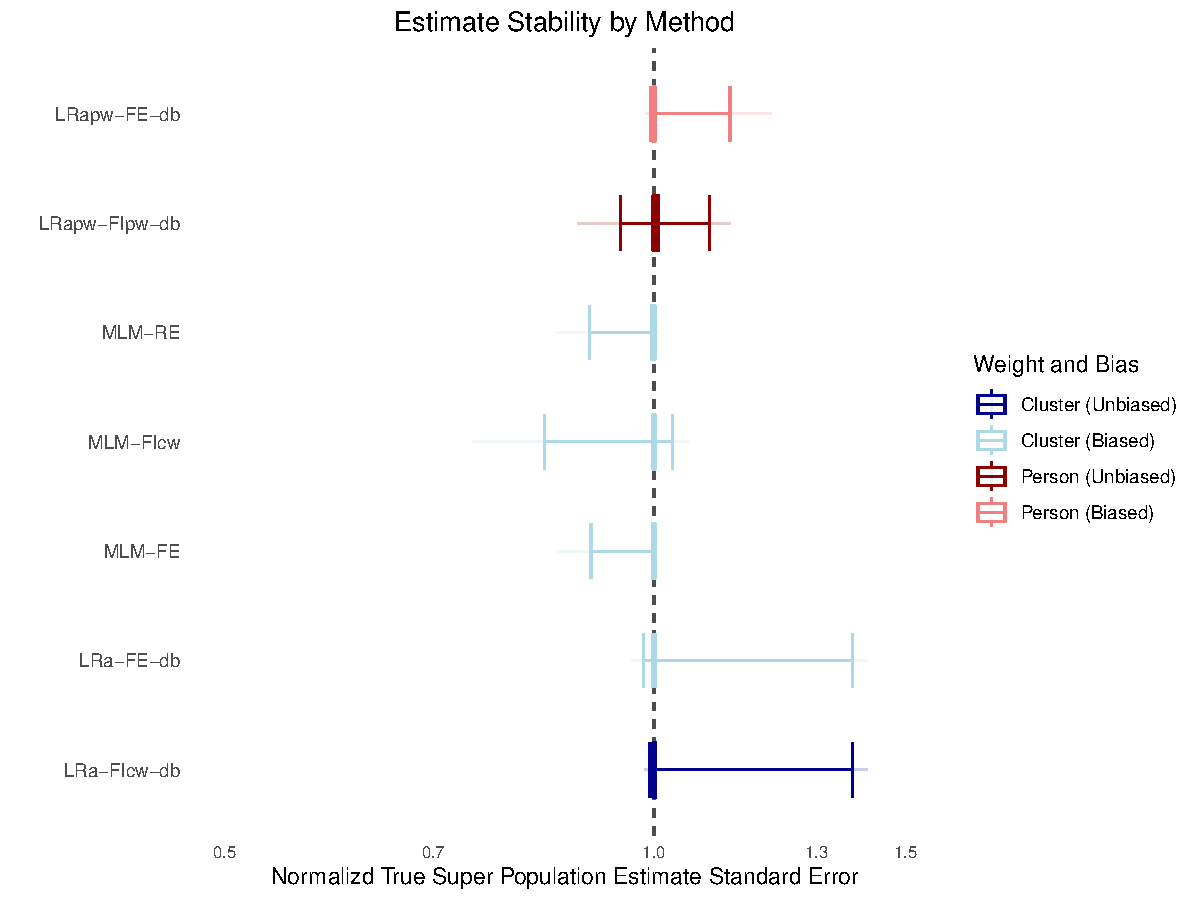
\includegraphics{Simulation-Memo-3_files/figure-latex/rmse-2} \end{center}

\subsection{What does the coverage look like for each
estimator}\label{what-does-the-coverage-look-like-for-each-estimator}

Coverage is the percentage of simulation replications where the
estimator is within the 95\% confidence interval. We would like the
number to 95\% (the boxplots have a red line at there). The notable
things are that the coverage for the MLM estimators is often very bad
but other than that the coverage for the cluster weighted estimators is
generally good. The coverage rates for the person weighted estimators
however are pretty bad across methods,it's either very low (meaning the
SEs are being underestimated) or too high (meaning the SEs are being
overestimated within the same methods. In addition, finite versus super
makes very little difference for the cluster targeted estimators but
makes a noticeable difference for the person weighted estimators.

\begin{center}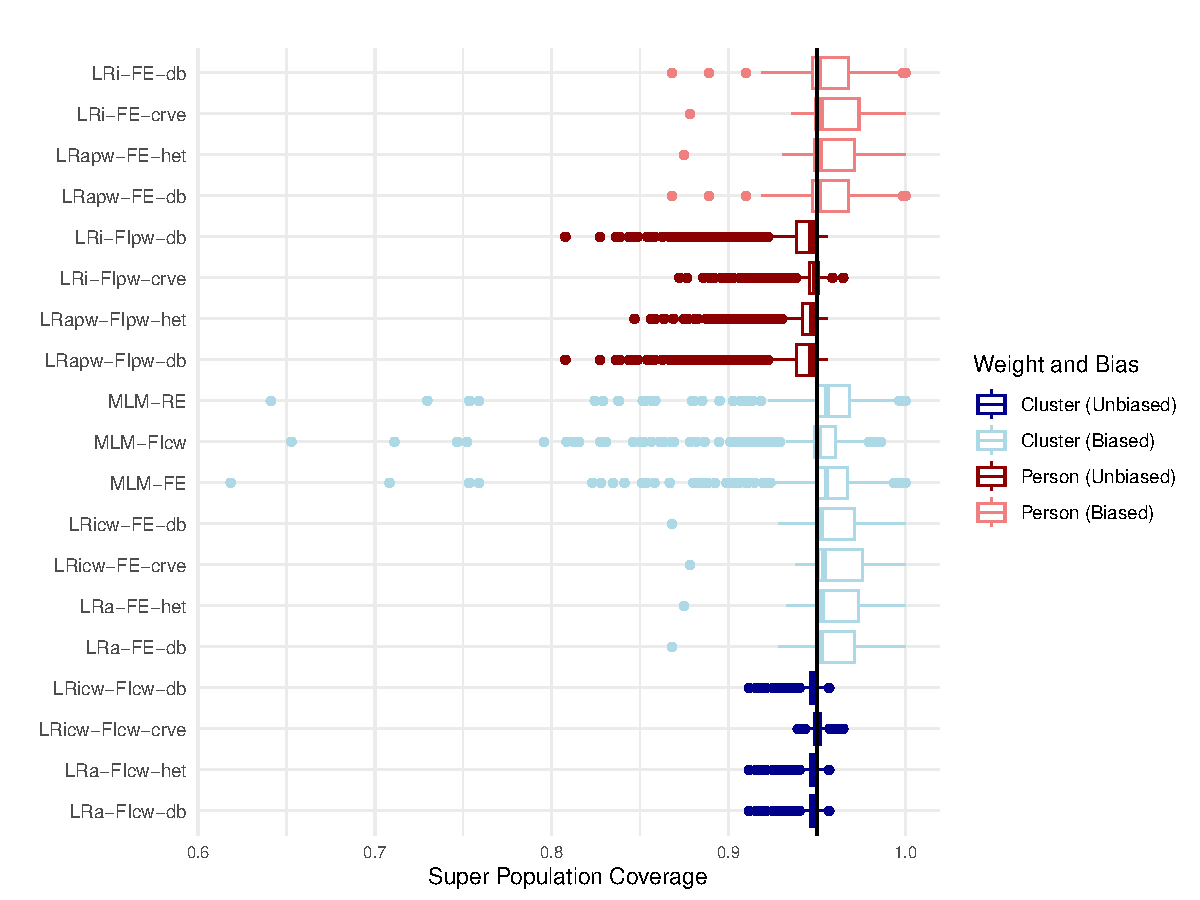
\includegraphics{Simulation-Memo-3_files/figure-latex/cov-1} \end{center}

\begin{center}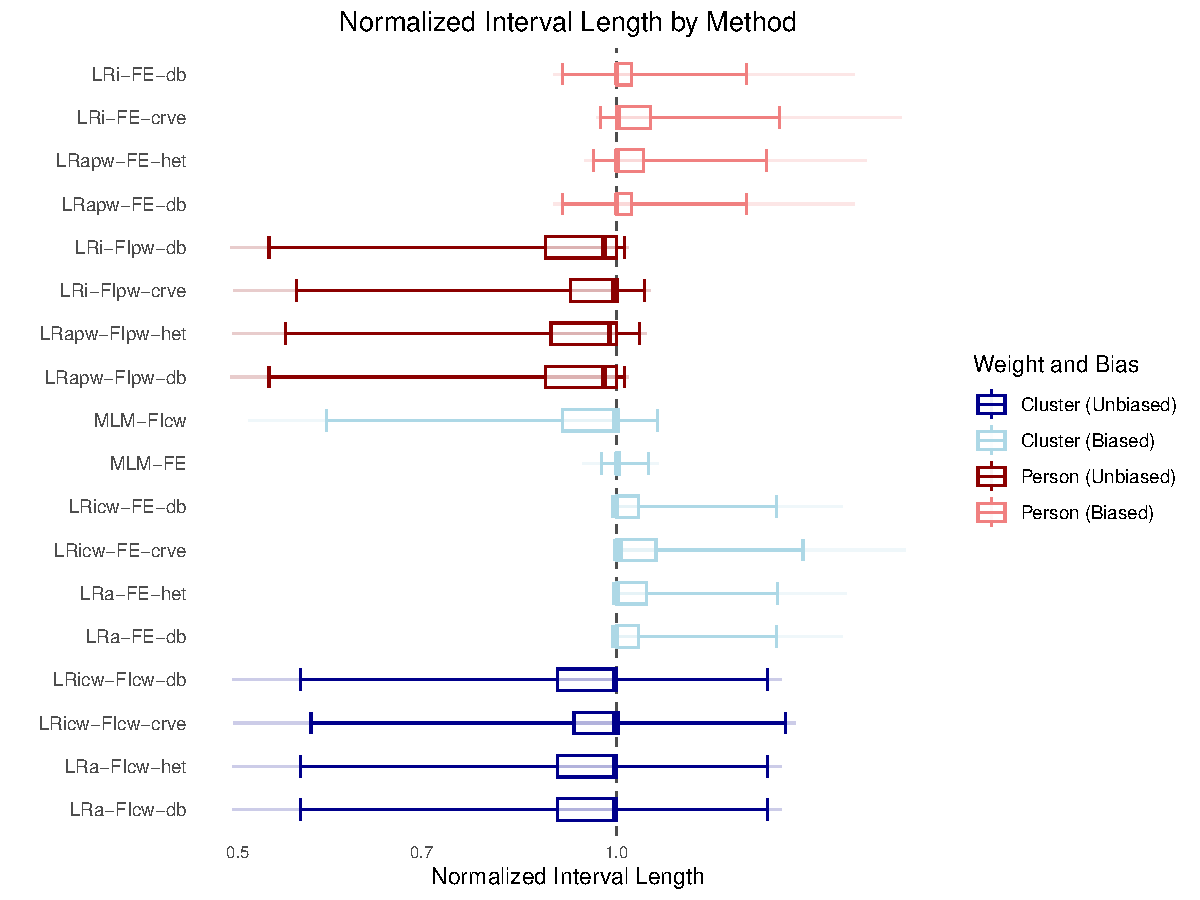
\includegraphics{Simulation-Memo-3_files/figure-latex/cov-2} \end{center}

\subsection{What do the standard errors look like for each
estimator}\label{what-do-the-standard-errors-look-like-for-each-estimator}

Standard error inflation is the ration of the estimated standard error
over the true standard error. High inflation means the standard errors
are too big and low inflation means the standard errors are too small.

For some of the methods the standard error estimates are way off, but it
does not seem obviously driven by low degrees of freedom. The true
finite standard errors do not look to be the same as the true super
standard errors.

\begin{center}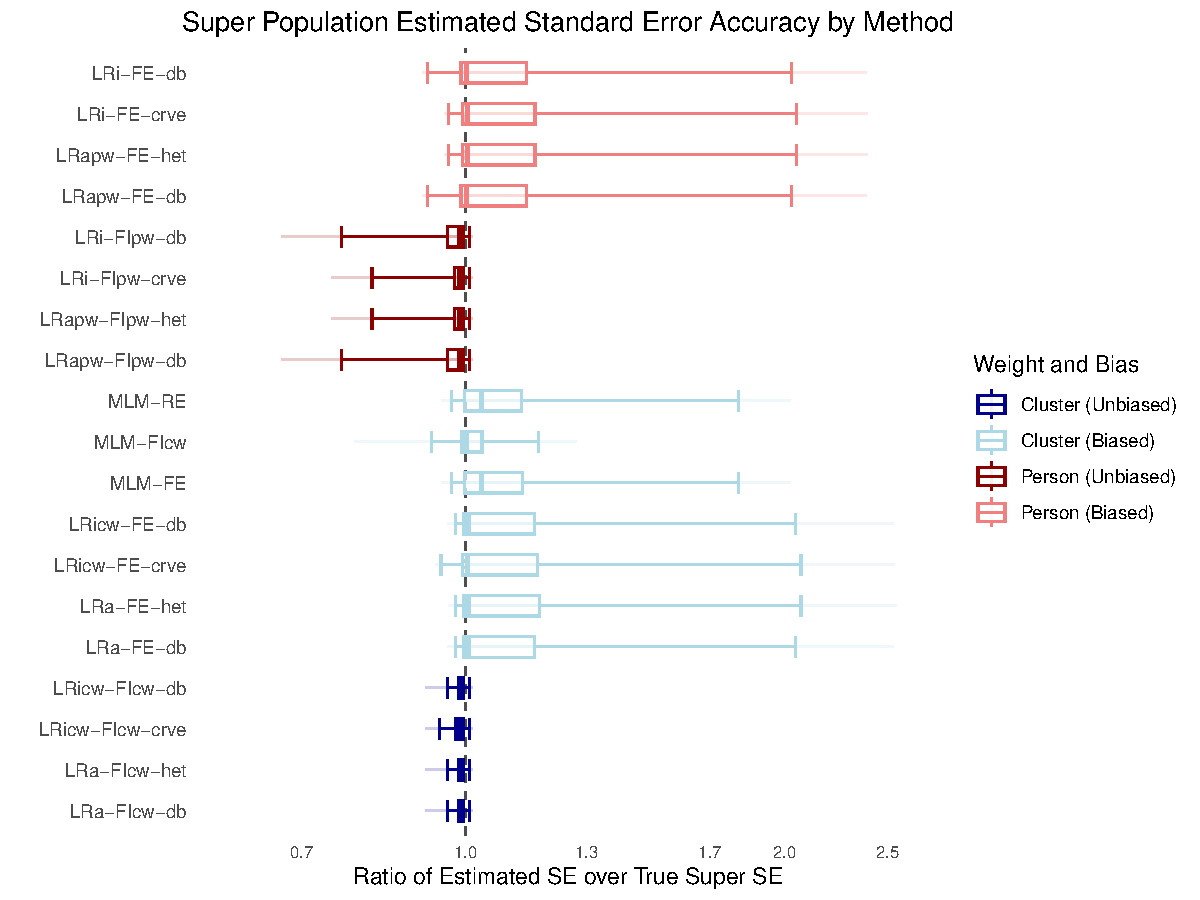
\includegraphics{Simulation-Memo-3_files/figure-latex/infl-1} \end{center}

\begin{center}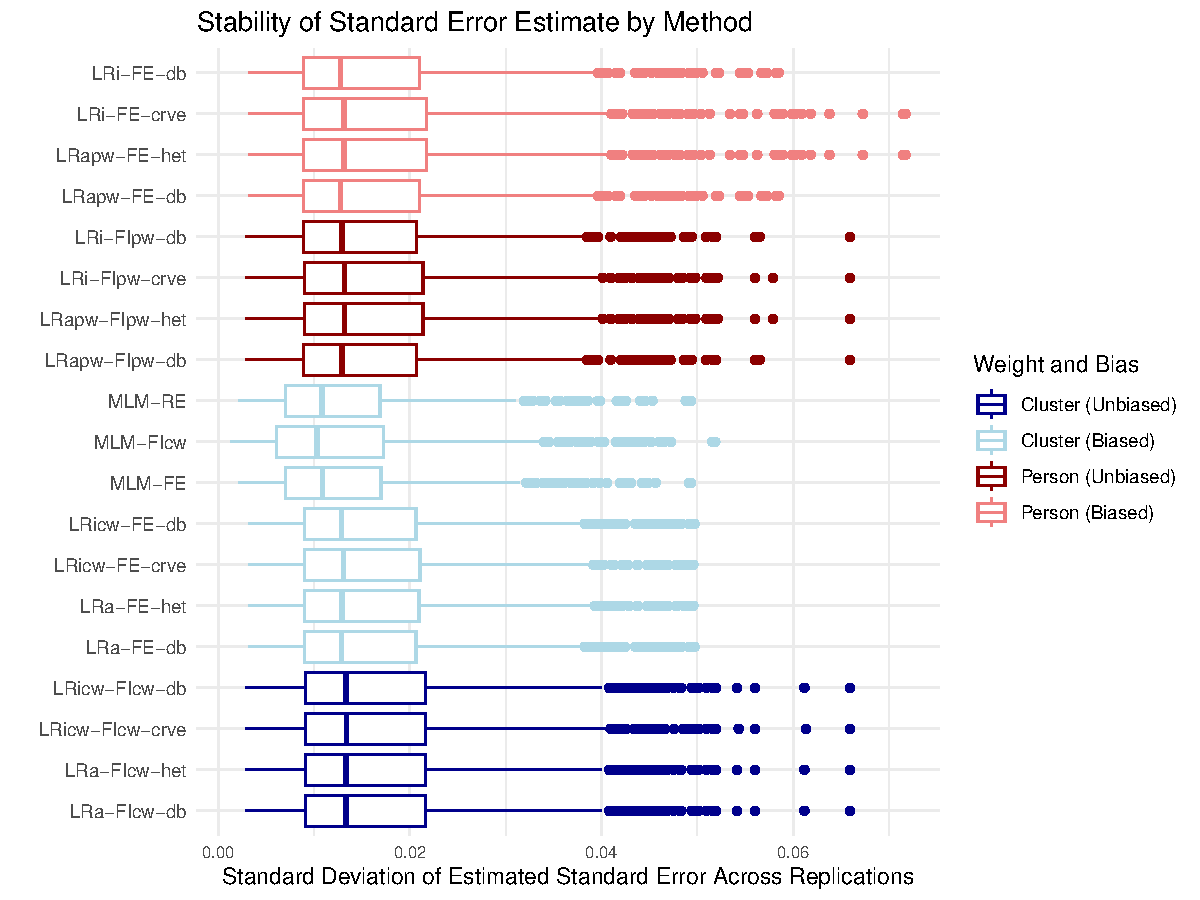
\includegraphics{Simulation-Memo-3_files/figure-latex/infl-2} \end{center}

======================================= Model for method: LRa-FE-db
Number of observations: 1296 R-squared: 0.7457939
=======================================

======================================= Model for method: LRa-FE-het
Number of observations: 1296 R-squared: 0.7486725
=======================================

======================================= Model for method: LRa-FIcw-db
Number of observations: 1296 R-squared: 0.728729
=======================================

======================================= Model for method: LRapw-FE-db
Number of observations: 1296 R-squared: 0.769057
=======================================

======================================= Model for method: LRapw-FE-het
Number of observations: 1296 R-squared: 0.7735951
=======================================

======================================= Model for method: LRapw-FIpw-db
Number of observations: 1296 R-squared: 0.7566025
=======================================

======================================= Model for method: LRapw-FIpw-het
Number of observations: 1296 R-squared: 0.7626567
=======================================

======================================= Model for method: LRicw-FE-crve
Number of observations: 1296 R-squared: 0.7464338
=======================================

======================================= Model for method:
LRicw-FIcw-crve Number of observations: 1296 R-squared: 0.7279335
=======================================

======================================= Model for method: MLM-FE Number
of observations: 1296 R-squared: 0.7635452
=======================================

======================================= Model for method: MLM-FIcw
Number of observations: 1296 R-squared: 0.7863796
=======================================

======================================= Model for method: MLM-RE Number
of observations: 1296 R-squared: 0.7647602
=======================================

\begin{verbatim}
                                  term LRa-FE-db LRa-FE-het LRa-FIcw-db
\end{verbatim}

1 (Intercept) 0.01*** 0.01*** 0.01\textbf{\emph{ 2 block\_typeS 0.00
0.00 0.00 3 block\_typeL 0.01}} 0.01*** 0.00\textbf{ 4 J.barS -0.00}
-0.00** -0.00\textbf{ 5 J.barL -0.01}* -0.01*** -0.01\textbf{\emph{ 6
size.impact.cor.schoolL -0.00 -0.00 -0.00 7 sd.schoolL 0.00}} 0.00***
0.00\textbf{\emph{ 8 ICC.schoolL 0.01}} 0.01*** 0.01\textbf{\emph{ 9
variable.nTRUE 0.00} 0.00* 0.00. 10 cv.schoolS 0.00 0.00 0.00 11
cv.schoolL 0.00* 0.00. 0.00. 12 num.cov.schoolS -0.00 -0.00 -0.00 13
num.cov.schoolL -0.00 -0.00 0.00 14 block\_typeS:J.barS -0.00 -0.00
-0.00 15 block\_typeL:J.barS -0.00 -0.00 0.00 16 block\_typeS:J.barL
-0.00 -0.00 -0.00 17 block\_typeL:J.barL -0.00}* -0.00*** -0.00\emph{ 18
block\_typeS:size.impact.cor.schoolL -0.00 -0.00 -0.00 19
block\_typeL:size.impact.cor.schoolL 0.00 0.00 0.00 20
block\_typeS:sd.schoolL 0.00 0.00 0.00 21 block\_typeL:sd.schoolL 0.00
0.00 0.00 22 block\_typeS:ICC.schoolL -0.00 -0.00 -0.00 23
block\_typeL:ICC.schoolL 0.00}** 0.00*** 0.01\emph{\textbf{ 24
block\_typeS:variable.nTRUE 0.00 0.00 0.00 25
block\_typeL:variable.nTRUE 0.00 0.00 0.00 26 block\_typeS:cv.schoolS
-0.00 -0.00 -0.00 27 block\_typeL:cv.schoolS 0.00 0.00 0.00 28
block\_typeS:cv.schoolL -0.00 -0.00 -0.00 29 block\_typeL:cv.schoolL
0.00 0.00 0.00} 30 block\_typeS:num.cov.schoolS 0.00 0.00 0.00 31
block\_typeL:num.cov.schoolS -0.00 -0.00 -0.00 32
block\_typeS:num.cov.schoolL 0.00 0.00 0.00 33
block\_typeL:num.cov.schoolL -0.00 -0.00 -0.00 34
J.barS:size.impact.cor.schoolL -0.00 -0.00 -0.00 35
J.barL:size.impact.cor.schoolL -0.00 -0.00 -0.00 36 J.barS:sd.schoolL
-0.00 -0.00 -0.00 37 J.barL:sd.schoolL -0.00 -0.00 -0.00 38
J.barS:ICC.schoolL -0.00}** -0.00*** -0.00\textbf{\emph{ 39
J.barL:ICC.schoolL -0.01}} -0.01*** -0.01\textbf{\emph{ 40
J.barS:variable.nTRUE -0.00 -0.00 -0.00 41 J.barL:variable.nTRUE -0.00}
-0.00* -0.00\emph{ 42 J.barS:cv.schoolS 0.00 0.00 0.00 43
J.barL:cv.schoolS -0.00 -0.00 -0.00 44 J.barS:cv.schoolL -0.00. -0.00.
-0.00. 45 J.barL:cv.schoolL -0.00} -0.00* -0.00} 46
J.barS:num.cov.schoolS 0.00 0.00 0.00 47 J.barL:num.cov.schoolS 0.00
0.00 0.00 48 J.barS:num.cov.schoolL -0.00 -0.00 -0.00 49
J.barL:num.cov.schoolL -0.00 -0.00 -0.00 50
size.impact.cor.schoolL:sd.schoolL -0.00 -0.00 0.00 51
size.impact.cor.schoolL:ICC.schoolL 0.00* 0.00* 0.00. 52
size.impact.cor.schoolL:variable.nTRUE 0.00* 0.00* 0.00\emph{ 53
size.impact.cor.schoolL:cv.schoolS 0.00 0.00 -0.00 54
size.impact.cor.schoolL:cv.schoolL 0.00 0.00 0.00 55
size.impact.cor.schoolL:num.cov.schoolS 0.00 0.00 0.00 56
size.impact.cor.schoolL:num.cov.schoolL 0.00 0.00 0.00 57
sd.schoolL:ICC.schoolL -0.00\textbf{ -0.00} -0.00} 58
sd.schoolL:variable.nTRUE -0.00* -0.00* -0.00\emph{ 59
sd.schoolL:cv.schoolS -0.00\textbf{ -0.00} -0.00} 60
sd.schoolL:cv.schoolL -0.00* -0.00* -0.00\emph{ 61
sd.schoolL:num.cov.schoolS 0.00 0.00 -0.00 62 sd.schoolL:num.cov.schoolL
-0.00 -0.00 0.00 63 ICC.schoolL:variable.nTRUE -0.00} -0.00* -0.00\emph{
64 ICC.schoolL:cv.schoolS -0.00 -0.00 0.00 65 ICC.schoolL:cv.schoolL
-0.00}** -0.00*** -0.00\textbf{\emph{ 66 ICC.schoolL:num.cov.schoolS
-0.00 -0.00 -0.00 67 ICC.schoolL:num.cov.schoolL -0.00 -0.00 -0.00 68
variable.nTRUE:cv.schoolS -0.00 -0.00 -0.00 69 variable.nTRUE:cv.schoolL
0.00}} 0.00*** 0.01\textbf{\emph{ 70 variable.nTRUE:num.cov.schoolS
-0.00} -0.00* -0.00\emph{ 71 variable.nTRUE:num.cov.schoolL -0.00 -0.00
-0.00 72 cv.schoolS:num.cov.schoolS 0.00. 0.00. 0.00} 73
cv.schoolL:num.cov.schoolS 0.00* 0.00* 0.00\emph{ 74
cv.schoolS:num.cov.schoolL 0.00 0.00 0.00 75 cv.schoolL:num.cov.schoolL
0.00 0.00 0.00 LRapw-FE-db LRapw-FE-het LRapw-FIpw-db LRapw-FIpw-het
LRicw-FE-crve 1 0.01}} 0.01*** 0.01*** 0.01*** 0.01\textbf{\emph{ 2 0.00
0.00 0.00 0.00 0.00 3 0.00}} 0.00*** 0.00*** 0.00** 0.01\textbf{\emph{ 4
-0.00} -0.00. -0.00} -0.00** -0.00\textbf{ 5 -0.00}* -0.00** -0.01***
-0.01*** -0.01\textbf{\emph{ 6 -0.00 -0.00 -0.00 -0.00 -0.00 7 0.00}}
0.00*** 0.00*** 0.00*** 0.00\textbf{\emph{ 8 0.01}} 0.01*** 0.01***
0.01*** 0.01\textbf{\emph{ 9 -0.00 -0.00 -0.00 -0.00 0.00} 10 -0.00
-0.00 -0.00 -0.00 0.00 11 -0.00. -0.00. -0.00 -0.00 0.00\emph{ 12 -0.00
-0.00 -0.00 -0.00 -0.00 13 0.00 0.00 0.00 0.00 -0.00 14 -0.00 -0.00
-0.00 -0.00 -0.00 15 -0.00 -0.00 0.00 0.00 -0.00 16 -0.00 -0.00 -0.00
-0.00 -0.00 17 -0.00}} -0.00*** -0.00* -0.00. -0.00\textbf{\emph{ 18
-0.00 -0.00 -0.00 -0.00 -0.00 19 0.00 0.00 0.00 0.00 0.00 20 0.00 0.00
0.00 0.00 0.00 21 0.00 0.00 0.00 0.00 0.00 22 -0.00 -0.00 -0.00 -0.00
-0.00 23 0.00}} 0.00*** 0.00*** 0.00*** 0.00\textbf{\emph{ 24 0.00 0.00
0.00 0.00 0.00 25 0.00}} 0.00*** -0.00 -0.00 0.00 26 0.00 0.00 -0.00
-0.00 -0.00 27 0.00. 0.00. 0.00 0.00 0.00 28 0.00 0.00 -0.00 -0.00 -0.00
29 0.00*** 0.00*** 0.00 0.00 0.00 30 0.00 0.00 0.00 0.00 0.00 31 -0.00
-0.00 -0.00 -0.00 -0.00 32 0.00 0.00 0.00 0.00 0.00 33 -0.00 -0.00 -0.00
-0.00 -0.00 34 -0.00 -0.00 -0.00 -0.00 -0.00 35 -0.00 -0.00 -0.00 -0.00
-0.00 36 -0.00 -0.00 -0.00 -0.00 -0.00 37 -0.00 -0.00 -0.00 -0.00 -0.00
38 -0.00*** -0.00*** -0.00*** -0.00*** -0.00\textbf{\emph{ 39 -0.01}}
-0.01*** -0.01*** -0.01*** -0.01\textbf{\emph{ 40 -0.00 -0.00 0.00 0.00
-0.00 41 -0.00} -0.00}* -0.00 -0.00. -0.00\emph{ 42 0.00 -0.00 0.00 0.00
0.00 43 -0.00 -0.00 0.00 -0.00 -0.00 44 -0.00 -0.00} -0.00 -0.00 -0.00.
45 -0.00* -0.00*** -0.00 -0.00. -0.00\emph{ 46 0.00 0.00 0.00 0.00 0.00
47 0.00 0.00 0.00 0.00 0.00 48 -0.00 -0.00 -0.00 -0.00 -0.00 49 -0.00
-0.00 -0.00 -0.00 -0.00 50 -0.00 -0.00 -0.00 -0.00 -0.00 51 0.00} 0.00*
0.00. 0.00. 0.00\emph{ 52 0.00 0.00. 0.00. 0.00. 0.00} 53 0.00 0.00
-0.00 -0.00 0.00 54 0.00 0.00 0.00 0.00 0.00 55 0.00 0.00 0.00 0.00 0.00
56 0.00 0.00 0.00 0.00 0.00 57 -0.00*** -0.00** -0.00*** -0.00***
-0.00\textbf{ 58 -0.00 -0.00 -0.00 -0.00 -0.00\emph{ 59 -0.00} -0.00*
-0.00* -0.00* -0.00} 60 -0.00 -0.00 -0.00 -0.00 -0.00\emph{ 61 0.00 0.00
-0.00 -0.00 0.00 62 -0.00 -0.00 0.00 -0.00 -0.00 63 0.00}** 0.00***
0.00*** 0.00*** -0.00\textbf{ 64 0.00 0.00 0.00 0.00 -0.00 65 0.00}*
0.00*** 0.00* 0.00** -0.00\textbf{\emph{ 66 -0.00 -0.00 -0.00 -0.00
-0.00 67 -0.00 -0.00 -0.00 -0.00 -0.00 68 0.00} 0.00} 0.00 0.00 -0.00 69
0.01*** 0.01*** 0.00*** 0.00*** 0.00\textbf{\emph{ 70 -0.00} -0.00*
-0.00* -0.00* -0.00\emph{ 71 -0.00 -0.00 -0.00 -0.00 -0.00 72 0.00 0.00
0.00} 0.00* 0.00. 73 0.00* 0.00* 0.00* 0.00* 0.00\emph{ 74 0.00 0.00
0.00 0.00 0.00 75 0.00 0.00 0.00 0.00 0.00 LRicw-FIcw-crve MLM-FE
MLM-FIcw MLM-RE 1 0.01}} 0.01*** 0.01*** 0.01\emph{\textbf{ 2 0.00 0.00
0.00 0.00 3 0.00} 0.01}** 0.00 0.01\emph{\textbf{ 4 -0.00} -0.00} -0.00*
-0.00\emph{ 5 -0.01}** -0.00*** -0.00*** -0.00\textbf{\emph{ 6 -0.00
-0.00 -0.00 -0.00 7 0.00}} 0.01*** 0.01*** 0.01\textbf{\emph{ 8 0.01}}
0.01*** 0.02*** 0.01\textbf{\emph{ 9 0.00} 0.00 0.00 0.00 10 0.00 0.00
0.00 0.00 11 0.00* 0.00 0.00 0.00 12 -0.00 -0.00 -0.00 -0.00 13 0.00
-0.00 -0.00 -0.00 14 -0.00 -0.00 -0.00 -0.00 15 0.00 -0.00 0.00 -0.00 16
-0.00 -0.00 -0.00 -0.00 17 -0.00. -0.00}* -0.00 -0.00\textbf{\emph{ 18
-0.00 -0.00 -0.00 -0.00 19 0.00 0.00 0.00 0.00 20 0.00 -0.00 -0.00 -0.00
21 0.00 -0.00. 0.00 -0.00. 22 0.00 -0.00 0.00 -0.00 23 0.01}} 0.00
0.00*** 0.00 24 0.00 0.00 0.00 0.00 25 0.00 0.00 0.00 0.00 26 -0.00
-0.00 -0.00 -0.00 27 0.00 0.00 0.00 0.00 28 -0.00 -0.00 -0.00 -0.00 29
0.00* 0.00 0.00 0.00 30 0.00 0.00 0.00 0.00 31 -0.00 -0.00 -0.00 -0.00
32 0.00 0.00 0.00 0.00 33 -0.00 -0.00 -0.00 -0.00 34 -0.00 -0.00 -0.00
-0.00 35 -0.00 -0.00. -0.00* -0.00. 36 -0.00 -0.00* -0.00** -0.00\emph{
37 -0.00 -0.00}** -0.00*** -0.00\textbf{\emph{ 38 -0.00}} -0.00***
-0.01*** -0.00\textbf{\emph{ 39 -0.01}} -0.01*** -0.01***
-0.01\textbf{\emph{ 40 -0.00 -0.00 -0.00 -0.00 41 -0.00} -0.00 -0.00.
-0.00 42 0.00 0.00 0.00 0.00 43 -0.00 0.00 0.00 0.00 44 -0.00. -0.00
-0.00 -0.00 45 -0.00} -0.00 -0.00 -0.00 46 0.00 0.00 0.00 0.00 47 0.00
0.00 0.00 0.00 48 -0.00 0.00 0.00 0.00 49 -0.00 -0.00 -0.00 -0.00 50
0.00 -0.00 -0.00 -0.00 51 0.00. 0.00. 0.00. 0.00. 52 0.00* 0.00* 0.00*
0.00\emph{ 53 -0.00 0.00 0.00 0.00 54 0.00 0.00 0.00 0.00 55 0.00 0.00
0.00 0.00 56 0.00 0.00 0.00 0.00 57 -0.00} -0.00*** -0.00***
-0.00\textbf{\emph{ 58 -0.00} -0.00. -0.00 -0.00 59 -0.00* -0.00* -0.00.
-0.00. 60 -0.00* -0.00 -0.00 -0.00 61 -0.00 0.00 0.00 0.00 62 0.00 -0.00
-0.00 -0.00 63 -0.00} 0.00 0.00 0.00 64 -0.00 -0.00 -0.00 -0.00 65
-0.00*** -0.00 -0.00 -0.00 66 -0.00 -0.00 -0.00 -0.00 67 -0.00 -0.00
-0.00 -0.00 68 0.00 -0.00 0.00 -0.00 69 0.01*** 0.00 0.00* 0.00 70
-0.00* -0.00* -0.00. -0.00\emph{ 71 -0.00 -0.00 -0.00 -0.00 72 0.00}
0.00 0.00 0.00 73 0.00* 0.00* 0.00* 0.00* 74 0.00 0.00 -0.00 0.00 75
0.00 0.00 0.00 0.00 method sd.SE.hat.s sd.ATE size.impact.cor J.bar
sd.school 1 LRa-FE-db 0.04969950 L L 0 L 2 LRa-FE-db 0.04964257 L L 0 0
3 LRa-FE-db 0.04934965 L L 0 L 4 LRa-FE-db 0.04914330 L L 0 L 5
LRa-FE-db 0.04833746 L L S 0 6 LRa-FE-het 0.04958679 L L 0 L 7
LRa-FE-het 0.04945717 L L 0 0 8 LRa-FE-het 0.04934965 L L 0 L 9
LRa-FE-het 0.04914330 L L 0 L 10 LRa-FE-het 0.04903156 L L S 0 11
LRapw-FE-db 0.05849423 L L 0 L 12 LRapw-FE-db 0.05847556 L L 0 L 13
LRapw-FE-db 0.05820059 L L 0 0 14 LRapw-FE-db 0.05727228 L L 0 0 15
LRapw-FE-db 0.05686273 L L 0 0 16 LRapw-FE-het 0.07172370 L L 0 L 17
LRapw-FE-het 0.07150984 L L 0 L 18 LRapw-FE-het 0.07145919 L L 0 0 19
LRapw-FE-het 0.06726747 L L 0 0 20 LRapw-FE-het 0.06379074 L L 0 L 21
LRicw-FE-crve 0.04958679 L L 0 L 22 LRicw-FE-crve 0.04934965 L L 0 L 23
LRicw-FE-crve 0.04930498 L L 0 0 24 LRicw-FE-crve 0.04914330 L L 0 L 25
LRicw-FE-crve 0.04903156 L L S 0 26 MLM-FE 0.04934962 L L 0 L 27 MLM-FE
0.04914328 L L 0 L 28 MLM-FE 0.04565466 L L 0 0 29 MLM-FE 0.04485496 L L
0 L 30 MLM-FE 0.04478190 L L 0 L 31 MLM-FIcw 0.05187094 L L 0 L 32
MLM-FIcw 0.05157175 L L 0 L 33 MLM-FIcw 0.04722937 L L 0 L 34 MLM-FIcw
0.04718535 L L 0 0 35 MLM-FIcw 0.04653229 L L 0 L 36 MLM-RE 0.04931761 L
L 0 L 37 MLM-RE 0.04879479 L L 0 L 38 MLM-RE 0.04531317 L L 0 0 39
MLM-RE 0.04454339 L L 0 L 40 MLM-RE 0.04436160 L L 0 L 41 LRa-FIcw-db
0.06593430 L L S 0 42 LRa-FIcw-db 0.06117638 L L 0 L 43 LRa-FIcw-db
0.05601163 L L 0 L 44 LRa-FIcw-db 0.05414307 L L 0 L 45 LRa-FIcw-db
0.05193417 L L 0 L 46 LRapw-FIpw-db 0.06593430 L L S 0 47 LRapw-FIpw-db
0.05650179 L L 0 L 48 LRapw-FIpw-db 0.05601163 L L 0 L 49 LRapw-FIpw-db
0.05193417 L L 0 L 50 LRapw-FIpw-db 0.05187420 L L 0 L 51 LRapw-FIpw-het
0.06593430 L L S 0 52 LRapw-FIpw-het 0.05790380 L L 0 L 53
LRapw-FIpw-het 0.05601163 L L 0 L 54 LRapw-FIpw-het 0.05211906 L L 0 L
55 LRapw-FIpw-het 0.05193417 L L 0 L 56 LRicw-FIcw-crve 0.06593430 L L S
0 57 LRicw-FIcw-crve 0.06134810 L L 0 L 58 LRicw-FIcw-crve 0.05601163 L
L 0 L 59 LRicw-FIcw-crve 0.05431772 L L 0 L 60 LRicw-FIcw-crve
0.05193417 L L 0 L ICC.school cv.school num.cov.school proptx.impact.cor
size.intercept.cor 1 L S 0 L L 2 L S L L L 3 L 0 L L L 4 L 0 0 L L 5 L S
S L L 6 L S 0 L L 7 L S L L L 8 L 0 L L L 9 L 0 0 L L 10 L S S L L 11 L
L 0 L L 12 L L L L L 13 L L L L L 14 L L 0 L L 15 L S L L L 16 L L 0 L L
17 L L L L L 18 L L L L L 19 L L 0 L L 20 L L 0 L L 21 L S 0 L L 22 L 0
L L L 23 L S L L L 24 L 0 0 L L 25 L S S L L 26 L 0 L L L 27 L 0 0 L L
28 L L L L L 29 L S 0 L L 30 L L 0 L L 31 L 0 L L L 32 L 0 0 L L 33 L L
0 L L 34 L L L L L 35 L S 0 L L 36 L 0 L L L 37 L 0 0 L L 38 L L L L L
39 L L 0 L L 40 L S 0 L L 41 L S S L L 42 L L L L L 43 L S S L L 44 L L
0 L L 45 L S 0 L L 46 L S S L L 47 L L L L L 48 L S S L L 49 L S 0 L L
50 L 0 L L L 51 L S S L L 52 L L L L L 53 L S S L L 54 L L 0 L L 55 L S
0 L L 56 L S S L L 57 L L L L L 58 L S S L L 59 L L 0 L L 60 L S 0 L L
size.impact.cor.school block\_type 1 0 L 2 L L 3 L L 4 L L 5 0 L 6 0 L 7
L L 8 L L 9 L L 10 0 L 11 L L 12 L L 13 L L 14 L L 15 L L 16 L L 17 L L
18 L L 19 L L 20 0 L 21 0 L 22 L L 23 L L 24 L L 25 0 L 26 L L 27 L L 28
L L 29 0 L 30 L L 31 L L 32 L L 33 L L 34 L L 35 L L 36 L L 37 L L 38 L
L 39 L L 40 0 L 41 0 L 42 L L 43 0 L 44 L L 45 0 L 46 0 L 47 L L 48 0 L
49 0 L 50 L L 51 0 L 52 L L 53 0 L 54 L L 55 0 L 56 0 L 57 L L 58 0 L 59
L L 60 0 L

\begin{center}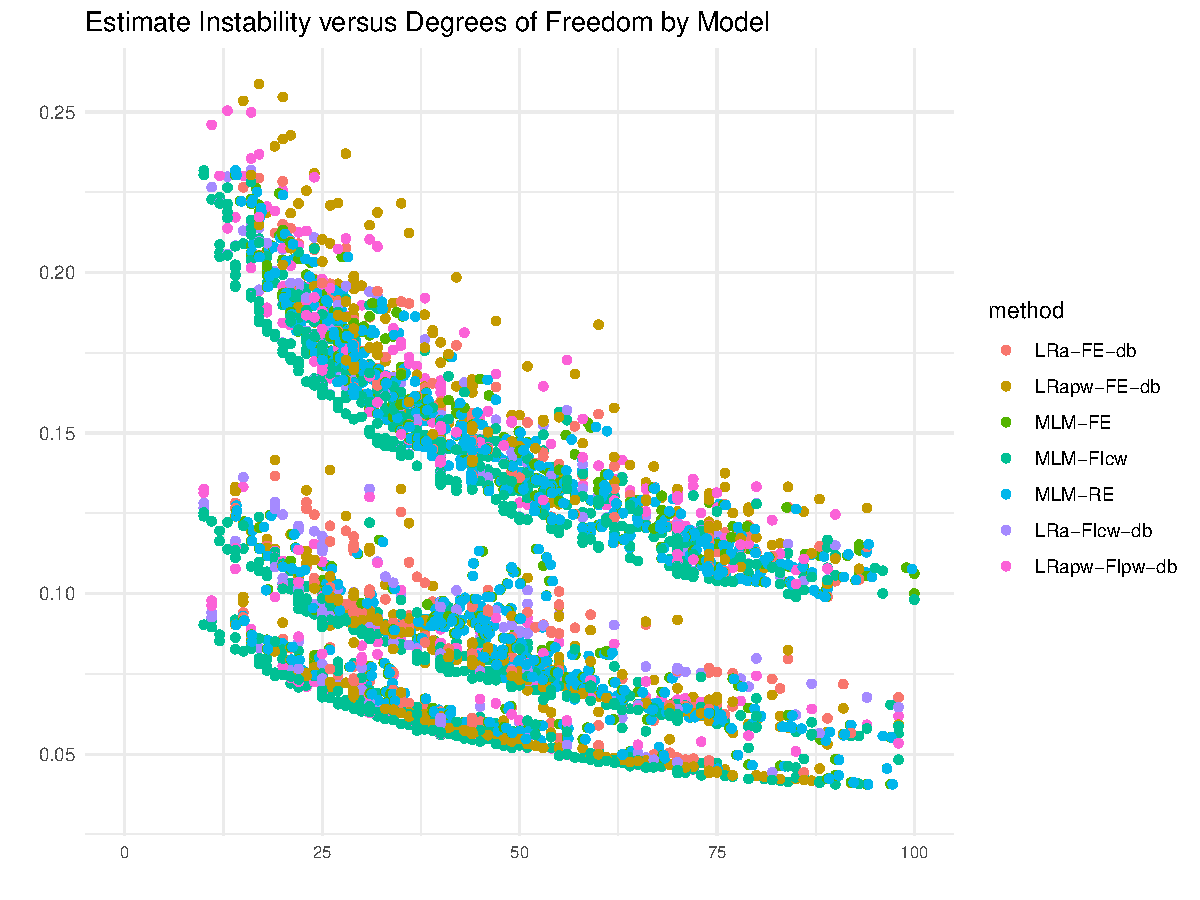
\includegraphics{Simulation-Memo-3_files/figure-latex/degfree-1} \end{center}

\begin{center}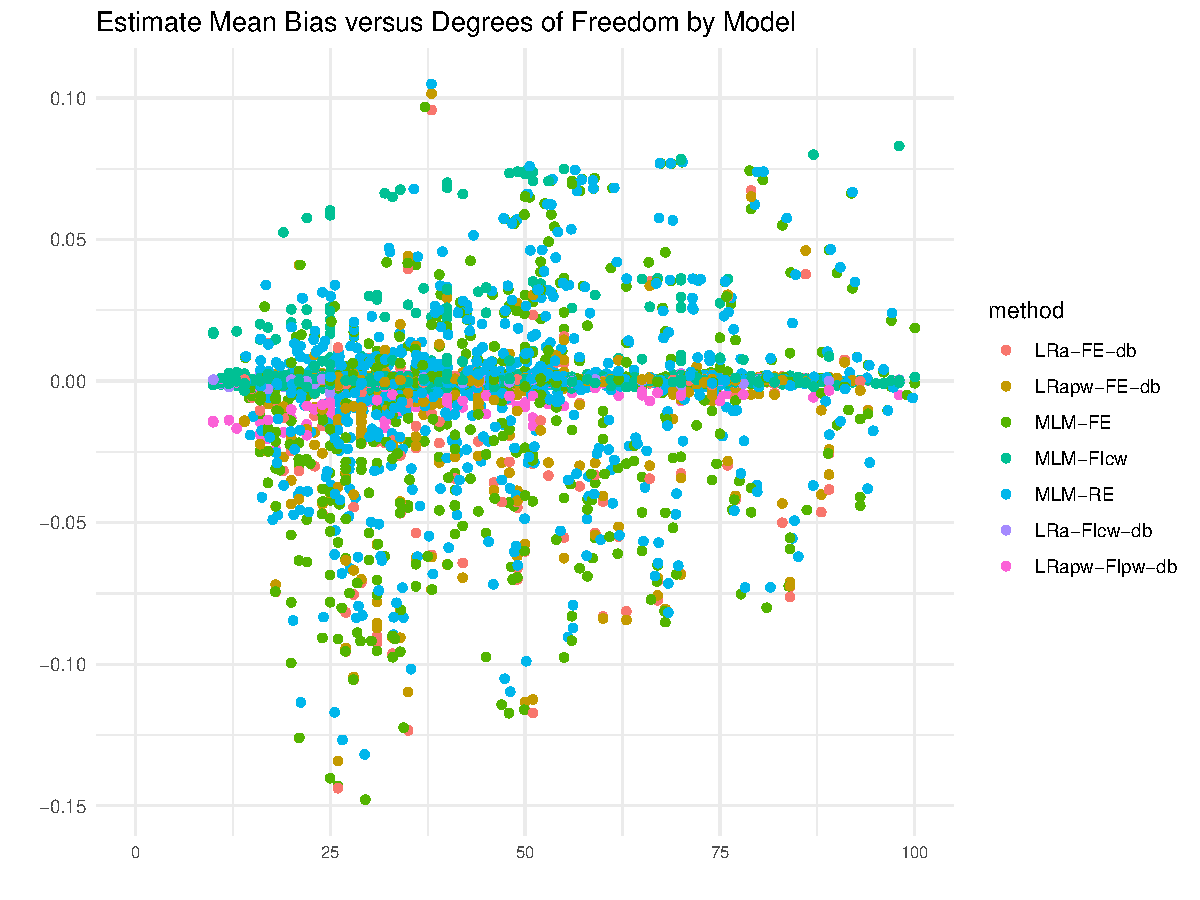
\includegraphics{Simulation-Memo-3_files/figure-latex/degfree-2} \end{center}

\end{document}
